\documentclass[conference]{IEEEtran}
\usepackage{cite}
\usepackage{amsmath,amssymb,amsfonts}
\usepackage{graphicx}
\usepackage{textcomp}
\usepackage{xcolor}
\usepackage{multicol}
\usepackage{float}
\usepackage[spanish]{babel}
\usepackage[spanish,vlined,ruled,]{algorithm2e}

\def\BibTeX{{\rm B\kern-.05em{\sc i\kern-.025em b}\kern-.08em
    T\kern-.1667em\lower.7ex\hbox{E}\kern-.125emX}}
\begin{document}

\title{Morphing}
\author{\IEEEauthorblockN{Joaquín Pérez Araya}
\IEEEauthorblockA{\textit{Departamento de Ciencias de la Computación} \\
\textit{Universidad de Chile}\\
Santiago, Chile \\
joaquin.perez.a@ug.uchile.cl}}


\maketitle

\begin{abstract}
	
\end{abstract}
 

\section*{Introducción} % ***Así la cosa no me molesta con los numeritos***
	El morphing es el efecto visual el cual se produce al cambiar una imagen a otra con un efecto de metamorfosis, actualmente se utiliza principalmente para el entretenimiento. En este documento se implementará el algoritmo descrito por Beier-Neely, que consiste en utilizar líneas de correspondencia entre la imagen de partida y la imagen de destino para describir la forma en que la mutación se va a llevar a cabo. Primero se describirá el diseño 
	
	
\section*{Diseño e Implementación}
	El código implementado se define en 3 funciones las cuales están implementadas en \texttt{morphing.py}: \textit{warp}, \textit{morph} y \textit{create morphing video}: La transformación de una imagen según un par de conjuntos de líneas (\textit{warp}), la creación de múltiples imágenes que son las que forman parte del morphing (\textit{morph}) y finalmente la creación, a partir de las imágenes calculadas en el proceso anterior el vídeo que muestra el cambio de las imágenes a lo largo del tiempo \textit{create morphing video}. También se dispone de un módulo adicional llamado \texttt{util.py} el cual contiene funciones auxiliares.
	
	\subsection*{Warpping}
		Para el warpping se utiliza el algoritmo propuesto por (paper), que está especificado en el Algoritmo 1:

	\begin{algorithm}[ht]
		\caption{Warpping}	
		\KwData{$image$ imagen fuente, $lines_{src}$ líneas fuente, $lines_{dst}$ líneas de destino.}
		\KwResult{Imagen que corresponde a la imagen fuente modificada según las líneas dadas.}
		\DontPrintSemicolon \;
		$destinationImage = zeros(shape(image)) $ \;
		\For{$pixel$ in $image$}{
			$DSUM = (0,0)$ \;
			$weightsum = 0$ \;
			\For{Line $P_i Q_i$ in $lines_{src}$ and $ P_i^{\prime} Q_i^{\prime}$ in $lines_{dst}$}{
			$u, v = calculate\_u\_v(X,P_i, Q_i)$ \;
			$X^\prime = calculate\_X^\prime (u,v,P_i^{\prime}, Q_i^{\prime})$ \;
			}		
		}}
		\KwRet{$h$}
		\label{asdf}
		\end{algorithm} 


		En el módulo de utilidades, están implementadas las funciones para el cálculo de $u$, $v$, $X^\prime$
	
	
	La implementación usa el algoritmo en su versión de mapeo inverso, es decir durante la ejecución se recorre la imagen de destino calculando qué pixeles de la imagen original deberían estar allí utilizando interpolación bilineal de los pixeles más cercanos de la imagen original, este método ofrece más simplicidad dado que se conoce los pixeles de destino de antemano por lo que el único inconveniente es el caso de que se requieren píxeles fuera de la imagen original por lo que se interpola según los pixeles ya calculados anteriormente, en cuyo caso sería:
		\begin{itemize}
               	\item Si se está en el primer pixel de la imagen, el de la esquina superior izquierda, éste se calcula como el pixel del mismo punto de la imagen de origen.
               	\item Si se está en la fila superior, se calcula usando el pixel anterior calculado, el de la izquierda de éste.
               	\item Si se está en la columna de la izquierda, se calcula usando el pixel de la fila superior.
               	\item Si se está en la columna de la derecha, se calcula utilizando los 3 pixeles que están cercanos a éste: Superior izquierdo, superior e izquierdo.
               	\item De otra forma se calcula utilizando 4 pixeles cercanos: Superior izquierdo, superior, superior derecho e izquierdo.
		\end{itemize}
	
	\subsection*{Morphing}
	
	\subsection*{Video}



\section*{Experimentación}
	Se realizaron pruebas con los siguientes valores para medir los pesos	
	
\section*{Conclusión}
	La técnica implementada de Morphing, es bastante lenta, dado que su tiempo de ejecución aumenta según la cantidad de píxeles, la cantidad de líneas determinadas y la cantidad de imágenes totales que se quieren, sin embargo esto otorga más control a la hora de elegir la forma de cómo se va animando la imagen a lo largo del morphing completo.
	
\begin{thebibliography}{99}
	 \bibitem{Paper} 

\end{thebibliography}

\end{document}

\begin{figure}[H]
    \centering
    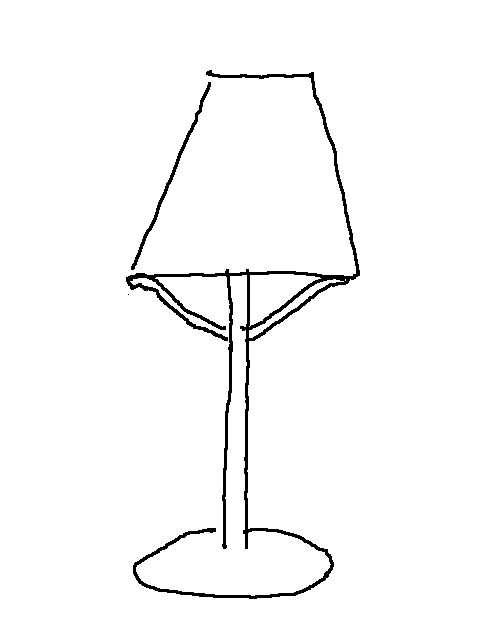
\includegraphics[width=0.95\linewidth]{image/lamps.jpg} \par

\caption{Ejemplo de una posible búsqueda, la imagen de la izquierda representa el dibujo de búsqueda y las de la derecha los resultados esperados.}
\end{figure}